\hypertarget{_s_c_p_i__lexer_8h}{\section{scpi/\-S\-C\-P\-I\-\_\-lexer.h File Reference}
\label{_s_c_p_i__lexer_8h}\index{scpi/\-S\-C\-P\-I\-\_\-lexer.\-h@{scpi/\-S\-C\-P\-I\-\_\-lexer.\-h}}
}
This graph shows which files directly or indirectly include this file\-:\nopagebreak
\begin{figure}[H]
\begin{center}
\leavevmode
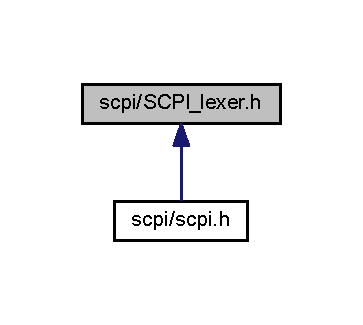
\includegraphics[width=174pt]{_s_c_p_i__lexer_8h__dep__incl}
\end{center}
\end{figure}


\subsection{Detailed Description}
The lexer performs a lexical analysis of a $ \langle$ P\-R\-O\-G\-R\-M\-A M\-E\-S\-S\-A\-G\-E $ \rangle$ , breaking it into its constituent headers command and parameter tokens and as such, forms the first stage of the parser. For further details on the parser see \hyperlink{_s_c_p_i__parser_8h}{S\-C\-P\-I\-\_\-parser.\-h}.

This file should not need to be edited by the user. 